\documentclass[10pt,letterpaper]{article}

% Packages
\usepackage[utf8]{inputenc}
\usepackage[top=0.85in,left=1.5in,footskip=0.75in]{geometry}
\usepackage{lastpage,fancyhdr,graphicx}
\usepackage{epstopdf}
\usepackage{verbatim}
\usepackage{amsmath}
\usepackage{amsfonts}
\usepackage{hyperref}
\usepackage{setspace}
\usepackage{algorithm}
\usepackage{algpseudocode}
\usepackage{hyperref}

% Text layout
\raggedright
\setlength{\parindent}{0.5cm}
\textwidth 5.5in 
\textheight 8.75in
\onehalfspacing

% Bibliography
% \usepackage[backend=biber,style=numeric,sorting=ynt]{biblatex}
% \addbibresource{bibliography.bib}

% C++ symbol
\newcommand{\CC}{C\nolinebreak\hspace{-.05em}\raisebox{.4ex}{\tiny\bf +}\nolinebreak\hspace{-.10em}\raisebox{.4ex}{\tiny\bf +}}
\def\CC{{C\nolinebreak[4]\hspace{-.05em}\raisebox{.4ex}{\tiny\bf ++}}}

% Header and footer
\pagestyle{fancy}
\fancyhf{}
\rfoot{\thepage/\pageref{LastPage}}
\renewcommand{\headrulewidth}{0pt}
\fancyheadoffset[L]{2.25in}
\fancyfootoffset[L]{2.25in}

\begin{document}
\bibliographystyle{plain}

\vspace*{0.2in}

\begin{centering}
{\Huge\textbf\newline{Pandemia: User Guide}}
\\
\bigskip

\includegraphics[width=0.2\textwidth]{pandemia_logo}
\\
\bigskip
\today
\\
\end{centering}

\tableofcontents

\section{Introduction}

Pandemia is an individual-based stochastic pandemic simulator. It simulates and visualizes the spread of an infectious disease across multiple geographical regions. These regions might represent the countries of the world, or the administrative divisions of a single country.

The software parallelizes computation over the regions, calculating the interactions between regions on a coarser timescale than the one used to discretize the individual-based simulations within each region. The user can specify a scale factor, adjusting the number of individuals, locations, and other relevant quantities appearing in each region. Pandemia is therefore fast and scalable, able to simulate extremely large numbers of individuals, while supporting a wide range of highly adaptable features.

This software will be of use to researchers looking to assess the impact of policy in the context of a public health emergency caused by an infectious disease of humans. The disease could, for example, be a respiratory infectious disease spread by a coronavirus or an influenza virus. The emergence and re-emergence of infectious diseases threatens the health and well-being of people all over the world. Tools such as Pandemia can play a vital role in supporting pandemic preparedness and response.

This user guide presents an overview of the model and its various components.

\section{Quick start}

Quick start / Install

\section{Inputs and Outputs}

Inputs and Outputs

\section{ABMlux}

Pandemia is based on the earlier ABMlux model, used for the article:
\begin{itemize}
\item[] J. Thompson and S. Wattam, \textit{Estimating the impact of interventions against COVID-19: From lockdown to vaccination}, PLOS ONE, 2021.
\end{itemize}
In that article, the authors presented an agent-based model of the COVID-19 pandemic in Luxembourg, and used it simulate the impact of interventions over the first 6 months of the pandemic. Pandemia is a far-reaching generalization of the ABMlux model. 

\section{World}

The Pandemia simulator acts upon a \textbf{World}. A \textbf{World} consists of \textbf{Regions}, with each \textbf{Region} consisting of \textbf{Agents}, \textbf{Locations} and \textbf{Activities}. Each agent performs a sequence of activities, and performs these activities in particular locations. A \textbf{World} additionally consists of a \textbf{Travel Matrix}, representing how many agents travel from each region to each other region each day. Here is the simplest possible \textbf{World} structure:
\begin{itemize}
\item One \textbf{Region}, one \textbf{Activity}, one \textbf{Location} and any number of \textbf{Agents}.
\end{itemize}
Here is the most complicated:
\begin{itemize}
\item Several \textbf{Regions}, with each \textbf{Region} consisting of several \textbf{Activities}, any number of \textbf{Locations} and any number of \textbf{Agents}, with a \textbf{Travel Matrix} describing the mixing between regions.
\end{itemize}

\subsection{Agents}
An individual human is referred to in the model as an \textbf{Agent}. Each agent is described by their age, a weekly routine of activities, locations at which the agent might perform these activities, and weights indicating the probabilities of these locations being chosen by that agent.

\subsection{Locations}
A \textbf{Location} represents, for example, an area of land or a building, such as a house, restaurant, shop or school classroom. A location is described by its type, for example House or Hospital, and a pair of spatial coordinates.

\subsection{Activities}
An \textbf{Activity} is something an agent does, for example cooking, driving to work, or shopping. Activities are simply labels, with no additional structure.

\subsection{Regions}
A \textbf{Region} represents, for example, a country or an administrative division of a country. A region consists of a set of activities, a set of agents, and a set of locations.

\subsection{World Factory}
A World is built by a \textbf{World Factory}. Different worlds can be obtained either by changing the configuration of a world factory, or by using a different world factory entirely.

\subsection{Vectorization}
Once a \textbf{World} has been built, it is then converted into a \textbf{Vector World}. This is done by converting each \textbf{Region} into a \textbf{Vector Region}. A \textbf{Vector Region} is a vectorized version of a \textbf{Region}, in which data is formatted as arrays of integers and floats, as opposed to Python lists and dictionaries. This facilitates interface with libraries of functions written in C.

\section{Simulator}

The Pandemia \textbf{Simulator} is the object that performs the pandemic simulation. Global parameters include the aforementioned scale factor, a random seed and the option of whether or not to parallelize the computation. The \textbf{Simulator} consists of a \textbf{Clock}, which represents time, a \textbf{World} and a number of \textbf{Components} and \textbf{Reporters}.

\subsection{Clock}

The \textbf{Clock} keeps track of time. It is an iterator that counts forward in time by one day, with each day being subdivided into ticks. Some components update each tick, while others update only each day. Interactions between regions, for example, are calculated at the beginning of each day.

\subsection{World}

The \textbf{World} is an object of the type described in the previous section, consisting of regions, with the regions consisting of agents, locations and activities.

\subsection{Components}

The model features of a number of \textbf{Components}:
\begin{itemize}
\item \textbf{Movement}
\item \textbf{Health}
\item \textbf{Hospitalization}
\item \textbf{Testing and Contact Tracing}
\item \textbf{Vaccination}
\item \textbf{Seasonality}
\item \textbf{Travel}
\end{itemize}
Pandemia provides a default model for each component, and a void model in which the component is inactive. The details of these default models will be described in subsequent sections.

\subsection{Reporters}

A \textbf{Reporter} collects data from the simulation for output and visualization. The simulator contains a message bus that broadcasts data labelled by topic, for example on new infections and deaths, while reporters subscribed to these topics collect the data and organize it. Some reporters save CSV files, tabulating infections by country, strain and date. Others save PNG files, plotting infections and deaths. There are also reporters that provide real time visualization of the simulation, using shapefiles or grid data supplied for the regions in question. All relevant parameters, including the filepaths of the output data, are specified by the user in the configuration file.

\subsection{Simulator Factory}

The \textbf{Simulator Factory} builds the simulator. The first step is to build the clock and world. Having done so, the simulator factory can then be saved and reloaded. It is therefore not necessary to build a world every time a simulation is run. This is useful since building a world might be computationally intensive. The next step is to initialize the components and finally the reporters.

\subsection{Run}

Once the simulator has been built, it can then be run! The main Pandemia loop looks approximately as follows:

\begin{algorithm}
\caption{Main loop}\label{alg:mainloop}
\begin{algorithmic}
\Require clock, regions, travel{\_}matrix
\For{day in clock}
\State travel.dynamics(regions, travel{\_}matrix, day)
\For{region in regions}
\State seasonality.dynamics(region, day)
\State input.dynamics(region, day)
\For{tick in range(ticks{\_}in{\_}day)}
\State $\text{t} \gets (\text{ticks{\_}in{\_}day} * \text{day}) + \text{tick}$
\State health.dynamics(region, t)
\State movement.dynamics(region, t)
\State hospitalization.dynamics(region, t)
\EndFor
\State testing{\_}and{\_}contact{\_}tracing.dynamics(region, t)
\State vaccination.dynamics(region, t)
\EndFor
\EndFor
\end{algorithmic}
\end{algorithm}

Note that some components update each day, while others update each tick. At the beginning of each day, Pandemia decides who is travelling from each region to each other region, and infects these travellers based on the average infectiousness of their destination region. These travellers are then set aside for the remainder of the day. Pandemia then loops over the regions, performing independent agent-based simulations. Since for the remainder of the day these simulations are independent, the loop over the regions can be parallelized. In this way, Pandemia is both fast and scalable. On a laptop computer, using 15 CPUs and 24GB of RAM, Pandemia has been able to perform a 100 day simulation with 24 ticks per day, of over 100 million agents, in under 1.5 hours.

\section{Input}\label{sec:input}

The \textbf{Input} component allows the user to specify a \textbf{Policy}, consisting of interventions. A policy is encoded by arrays of integers and floats, indicating the availability or strength of various interventions in each region each day. Currently supported interventions include:
\begin{itemize}
\item \textbf{Lockdown}
\item \textbf{Border Closure}
\item \textbf{Vaccination}
\item \textbf{Testing and Contact Tracing}
\item \textbf{Quarantine}
\item \textbf{Face Masks}
\end{itemize}
The interventions are implemented inside the relevant components. For example, a lockdown is implemented within the movement component.

\section{Movement}

In the default movement model, each agent performs a sequence of activities and performs these activities at particular locations.

Recall that, during the building of the world, each agent is assigned a weekly routine consisting of a sequence of activities. It is assumed that these routines start on a Sunday. For example, suppose in a given region there are three activities, \textbf{Home}, \textbf{Work} and \textbf{School}, and that we wish to specify the routine of agents with an 8 hour time resolution. Then one weekly routine could be:
\begin{center}
[\textbf{Home}, \textbf{Home}, \textbf{Home}, \textbf{Home}, \textbf{Work}, \textbf{Home}, \textbf{Home}, \textbf{Work}, \textbf{Home}, \textbf{Home}, \textbf{Work}, \textbf{Home}, \textbf{Home}, \textbf{Work}, \textbf{Home}, \textbf{Home}, \textbf{Work}, \textbf{Home}, \textbf{Home}, \textbf{Home}, \textbf{Home}]
\end{center}
representing a typical working week, while another weekly routine could be:
\begin{center}
[\textbf{Home}, \textbf{Home}, \textbf{Home}, \textbf{Home}, \textbf{School}, \textbf{Home}, \textbf{Home}, \textbf{School}, \textbf{Home}, \textbf{Home}, \textbf{School}, \textbf{Home}, \textbf{Home}, \textbf{School}, \textbf{Home}, \textbf{Home}, \textbf{School}, \textbf{Home}, \textbf{Home}, \textbf{Home}, \textbf{Home}]
\end{center}
representing a typical school week.

Recall also, that during the building of the world, each agent is assigned a weighted set of locations for each activity. For example, suppose in a given region there are two activities, \textbf{Home} and \textbf{Other}. Then, a given agent might be assigned a single location for the activity \textbf{Home}, with weight $1.0$, and several other locations for the activity \textbf{Other}, with weights chosen according to the distance from home, so that locations further from home are less likely to be visited.

In the default movement model, whenever an agent switches from one activity to another, the agent randomly selects a new location from the corresponding set of locations, using the specified weights, at which they will then perform this new activity. Upon changing activity, agents may also put on or take off a face mask, depending on the activity and the current policy on face masks, as specified in the \textbf{Configuration} and \textbf{Input}. If the change of location is prohibited by a policy intervention, for example a lockdown, then the choice of agent is overridden and they are instead directed to their home location. In particular, each agent must for the default movement model be assigned a home location.

\section{Health}\label{sec:health}

Infectious disease models typically represent health using discrete states. In such a compartmental model, the population is partitioned into subsets, labelled \textit{Susceptible}, \textit{Infected}, \textit{Recovered} and \textit{Dead}. These compartments can then be subdivided, and new compartments added, to produce increasingly complicated models. This approach runs into difficulties once partial immunity is introduced, since the compartmental label \textit{Recovered} then becomes ambiguous. It runs into further difficulties once multiple strains of the pathogen are introduced, since then the label \textit{Susceptible} becomes ambiguous.

Pandemia therefore dispenses with the compartmental framework altogether, taking an entirely new approach to modelling individual health. In the default health model, the health of an individual is described by five attributes:
\begin{itemize}
\item \textbf{Strain}
\item \textbf{Disease}
\item \textbf{Infectiousness}
\item \textbf{Immunity (outer layer)}
\item \textbf{Immunity (inner layers)}
\end{itemize}
The immune system is represented using layers, with the outer layer determining whether or not an infection is blocked, and the inner layers determining the outcome for infections that are not blocked. A key innovation of Pandemia is that, for each individual, these five attributes are stored as \textit{functions}. The value of an attribute at time $\texttt{t}$ is given by evaluating the corresponding function at time $\texttt{t}$. During a simulation, the following variables store the values of these functions at the current time:
\begin{itemize}
\item \texttt{current{\_}strain}
\item \texttt{current{\_}disease}
\item \texttt{current{\_}infectiousness}
\item \texttt{current{\_}sigma{\_}immunity{\_}failure}
\item \texttt{current{\_}rho{\_}immunity{\_}failure}
\end{itemize}
The prefix \texttt{sigma{\_}} refers to the outer layer of the immune system, while the prefix \texttt{rho{\_}} refers to the inner layers.

\subsection{Strain}

For agent $\texttt{n}$, the variable $$\texttt{current{\_}strain[n]}$$ indicates whether or not agent $\texttt{n}$ is infected, and if so with which strain. The variable is an integer, taking values in the range $$\{\texttt{-1, 0, 1, 2, \ldots, S - 1}\}$$ where $\texttt{S}$ denotes the number of strains. If the agent is not infected, then $$\texttt{current{\_}strain[n] = -1}.$$ We assume that agents can only be infected with one strain at a time.

\subsection{Disease}

For agent $\texttt{n}$, the variable $$\texttt{current{\_}disease[n]}$$ indicates the extent to which agent $\texttt{n}$ is diseased. The variable is a float, taking values in the range $\texttt{[0,1]}.$ If the agent has no disease, then $$\texttt{current{\_}disease[n] = 0}.$$ If the agent is dead, then $$\texttt{current{\_}disease[n] = 1}.$$ Values close to $\texttt{1}$ represent severe disease, values close to $\texttt{0}$ represent mild disease. Values above a threshold represent symptomatic disease, values below the threshold represent asymptomatic disease. 

\subsection{Infectiousness}

For agent $\texttt{n}$, the variable $$\texttt{current{\_}infectiousness[n]}$$ indicates the extent to which agent $\texttt{n}$ is infectious. The variable is a float, taking non-negative values. If the agent is infected but not infectious, then $$\texttt{current{\_}infectiousness[n]} = 0.$$ If the agent is infected, then increasing the value of this variable increases the probability that the agent transmits strain $\texttt{current{\_}strain[n]}$ to other agents.

\subsection{Immunity (Outer Layer)}

For agent $\texttt{n}$ and strain $\texttt{s}$, the variable $$\texttt{current{\_}sigma{\_}immunity{\_}failure[n][s]}$$ represents the probability that the immune system of agent $\texttt{n}$ \textit{fails} to prevent an infection when exposed to strain $\texttt{s}$. Being a probability, this variable is therefore a float taking values in the range $\texttt{[0,1]}.$ Since this variable stores a failure probability, values closer to $\texttt{0}$ represent higher levels of protection.

\subsection{Immunity (Inner Layers)}

If sigma immunity fails, then the pathogen makes it past the outer layer of defence and an infection occurs. The pathogen now confronts a number of internal layers. Each layer has a probability of failing to stop the pathogen, with the outcome of the infection getting progressively worse the deeper the pathogen penetrates. This binary tree structure allows the user to parametrize, for example, the efficacy of a vaccine against symptomatic disease, severe disease and death. If the pathogen passes through all but the last internal layer, which is impenetrable, then the agent experiences the worst possible outcome.

For example, suppose the model is configured in such a way that there are two internal layers. Then, for a given agent, infected with a given strain, there are two possible outcomes. If the first internal layer fails to stop the pathogen, then the outcome will be the latter of the two outcomes. If the first internal layer is successful, then the outcome will be the former of the two outcomes. These two outcomes could, for example, be configured to represent recovery and death, respectively.

More generally, suppose the model is configured in such a way that there are $\texttt{R}$ internal layers, and therefore $\texttt{R}$ possible outcomes. Then, for agent $\texttt{n}$ and strain $\texttt{s}$, the variable $$\texttt{current{\_}rho{\_}immunity{\_}failure[n][s]}$$ gives a vector of probabilities, of length $\texttt{R}$, corresponding to the \textit{failure} probabilities of each layer. If a pathogen makes it past layer $\texttt{r}$, then it moves on to face layer $\texttt{r+1}$, else the agent gets outcome $\texttt{r}$. Since the last layer is impenetrable, the final entry in this vector is always equal to $\texttt{0}$, meaning that the last layer never fails to stop the pathogen.

The sampling of this binary tree structure occurs immediately after infection.

While sigma immunity determines whether or not an infection occurs, with rho immunity determining the outcome of that infection, to understand the outcomes themselves we must discuss the $\texttt{health{\_}presets}$.

\subsection{Presets and Updates}

The default response to an infection is determined for each agent, for each strain, during the initialization of the health component, before the start of the simulation. In particular, if an agent has been assigned the preset response $\texttt{p}$ from the set of possible presets $\texttt{health{\_}presets}$, then the object $\texttt{p[r]}$ contains data which determine updates, for each of the five health attributes described above, corresponding to outcome $\texttt{r}$.

For example, suppose that our model features two strains and two internal layers. Then the object $\texttt{p[r]}$ may be as follows:
\begin{center}
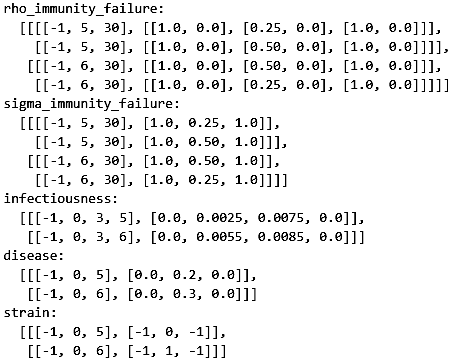
\includegraphics[width=0.5\textwidth]{codeexamplebw}
\end{center}

The numbers in these arrays encode step functions. For example, the pair of arrays $\texttt{[[-1,0,5], [0.0,0.2,0.0]]}$ encodes the step function $f$ given by
\begin{equation}
f(t) =
\begin{cases}
0.0 \text{ for } t < 0 \\
0.2 \text{ for } 5 > t \geq 0 \\
0.0 \text{ for } t \geq 5
\end{cases}.\nonumber
\end{equation}

Suppose in the above example that agent $\texttt{n}$ has just been infected with strain $\texttt{0}$, and that the infection has resulted in outcome $\texttt{r}$, with $\texttt{p[r]}$ as above. Then the variable $\texttt{current{\_}strain[n]}$ will take the value $\texttt{0}$ for the next $\texttt{5}$ days, after which it will return to the value $\texttt{-1}$, indicating that the agent is no longer infected. The variable $\texttt{current{\_}disease[n]}$ will take the value $\texttt{0.2}$ for the next $\texttt{5}$ days, after which it will return to the value $\texttt{0.0}$, indicating that the agent has recovered. The variable $\texttt{current{\_}infectiousness[n]}$ will take the value $\texttt{0.0025}$ for the next $\texttt{3}$ days, followed by $\texttt{0.0075}$ for $\texttt{2}$ days, after which it will return to the value $\texttt{0.0}$, indicating that the agent is no longer infectious.

Updates to the sigma and rho immunity variables are more complicated. The immunity variables are updated via the operation of function multiplication. Recall that the immunity functions store probabilities of failure, so the product of such functions give the probabilities of failure for overlapping immune responses, assuming independence.

Suppose in the above example that agent $\texttt{n}$ has no immunity against either strain prior to infection. Assume that the infection with strain $\texttt{0}$ occurred at time $\texttt{t}$. Then, after updating their immunity functions, the component of their sigma immunity function corresponding to strain $\texttt{0}$ will be given by the step function $$\texttt{[-1, t + 5, t + 30], [1.0, 0.25, 1.0]},$$ while the component corresponding to strain $\texttt{1}$ will be given by $$\texttt{[-1, t + 5, t + 30], [1.0, 0.5, 1.0]}.$$

In particular, for 25 days following the end of their infection, the probability that their immune system fails to protect against another infection by strain $\texttt{0}$ is improved from $\texttt{1.0}$ to $\texttt{0.25}$, after which it returns to $\texttt{1.0}$, representing a loss of immunity. The probability that their immune system fails to protect against an infection by strain $\texttt{0}$ is improved from $\texttt{1.0}$ to $\texttt{0.5}$, after which it returns to $\texttt{1.0}$, representing a loss of cross immunity.

Suppose now that at time $\texttt{t + 10}$ agent $\texttt{n}$ is again infected by strain $\texttt{0}$. Then between times $\texttt{t + 10}$ and $\texttt{t + 15}$, the three variables describing their current strain, disease and infectiousness will be updated as before. But the component of their sigma immunity function corresponding to strain $\texttt{0}$ will now be subject to appropriate multiplication, after which it will be given by the step function $$\texttt{[-1, t + 5, t + 15, t + 30, t + 40]},$$ $$\texttt{[1.0, 0.25, 0.0625, 0.25, 1.0]}.$$ In particular, between times $\texttt{t + 15}$ and $\texttt{t + 30}$ there are overlapping immunity responses, so that in order for a third infection to occur by strain $\texttt{0}$, the pathogen must overcome the immune response generated by the first infection \textit{and} the immune response generated by the second infection. Our assumption is that these events are independent, hence the multiplication of probabilities.

Updates to rho immunity are similar, except that these functions are now vector-valued, these vectors corresponding to the failure probabilities for each internal layer, meaning that the functions must be multiplied element-wise.

For a preset $\texttt{p}$ and outcome $\texttt{r}$, while the components of $\texttt{p[r]}$ corresponding to strain, disease and infectiousness each contain precisely $\texttt{S}$ functions, where $\texttt{S}$ is the number of strains, the components corresponding to rho and sigma immunity are containing precisely $\texttt{S} \times \texttt{S}$ functions, the additional dimension accounting for cross-immunity as in the above example.

\subsection{Transmission}

For a location $l$ in region $i$, we define:
\begin{equation*}
p_l := \left(1 - \prod_{m \in l} (1 - f_m)\right)
\end{equation*}
where $m \in l$ means all agents $m$ currently in location $l$, with
\begin{equation*}
f_m  := \omega_m\, \nu_m\, \mu(i)\, \lambda(l)\, \beta(s_m).
\end{equation*}
Here
\begin{itemize}
\item $\omega_m$ is the current face mask multiplier associated to agent $m$, which takes the value $1$ if they are not wearing a face mask, and some number smaller that $1$ if they are;
\item $\nu_m$ is the current infectiousness of agent $m$;
\item $\mu$ is a multiplier depending on the region $i$, reflecting for example seasonal changes in transmission that act on the regional level;
\item $\lambda$ is a multiplier depending on the location $l$, reflecting the fact that some types of location might be less conducive to transmission than others;
\item $\beta$ is a control coefficient depending on the strain $s_m$ that agent $m$ is currently infected with, if any.
\end{itemize}
For each susceptible agent $n$ in location $l$, with current face mask multiplier $\omega_n$, the probability that they are exposed at this time is then assumed to be $\omega_n p_l$. If such an agent is exposed, then to determine which strain they are exposed to, we assume the expression
\begin{equation*}
\frac{\sum_{\{m \in l: s_m = s\}} f_m}{\sum_{\{m \in l\}} f_m}
\end{equation*}
gives the probability that they are exposed to strain $s$. Given this exposure, the probability that they are actually infected with strain $s$ is then $\sigma_{ns}$, the current sigma immunity of agent $n$ against strain $s$. The outcome of this infection is then determined by the rho immunity of the agent, according the procedure outlined in the previous subsections.

\subsection{SIR Rescaling}

If the option $\texttt{sir{\_}rescaling}$ is set to $\texttt{True}$, then transmission probabilities are rescaled in such a way that approximates the homogeneous mixing of standard compartmental models. In particular, the $\texttt{sir{\_}rescaling}$ option multiplies all health model transmission probabilities by the reciprocal of the tick length, in days, divided by the number of agents in each location. Moreover, with this option activated it is also possible to implement a contact matrix, that can be used to represents differential mixing between population subgroups, for example age groups.

For example, suppose there is only one region, one location, one strain and no face masks. Suppose that $\nu_m = 1$ if $m$ is infected, with $\nu_m = 0$ otherwise. Denote by $N_{a}$ the number of people in group $a$ and by $h$ the step size (that is, the reciprocal of the tick length, in days). Then the $\texttt{sir{\_}rescaling}$ option multiplies all health model transmission probabilities by $h / N_a$. Denoting by $m_{ab}$ the mixing between groups $a$ and $b$ and by $I_b$ the number of currently infected agents in group $b$, for an agent $n$ in group $a(n)$, we have:
\begin{align} \nonumber
p_n =\, & 1 - \prod_{b} \left(1 - \frac{h \beta m_{a(n) b}}{N_b}\right)^{I_b} \\ \nonumber
\approx\, & 1 - \prod_{b \in A} \exp \left(-\frac{h\beta m_{a(n)b} I_b}{N_b}\right)\\ \nonumber
 = \, & 1 - \exp \left(- \sum_{b} \frac{h\beta m_{a(n)b} I_b}{N_b}\right)\\[2mm] \nonumber
 = \, & 1 - \exp \left(- h\beta (MI)_{a(n)}\right) \nonumber
\end{align}
where $M_{ab} := m_{ab} / N_b$ is the normalized contact matrix. This is consistent with a standard compartmental model, since the expected number of new infections in age group $a$ at time $t$ then satisfies the approximation
\begin{align} \nonumber
\mathbb{E}\left[\frac{S_a(t+h) - S_a(t)}{h}\right] \approx\, & -S_a(t)\left(\frac{1 - \exp \left(- h\beta (MI(t))_{a}\right)}{h}\right)\\[2mm] \nonumber
\approx\, & -\beta S_a(t) (MI(t))_a. \nonumber
\end{align}
In particular, with only one population subgroup we have $M = 1 / N$, therefore recovering the first equation
\begin{equation*}
\frac{d}{dt} S(t) = - \beta S(t)I(t) / N
\end{equation*}
of the SIR model. With exponentially distributed recovery times, and no reinfection, we recover the remaining equations, and therefore arrive at a stochastic approximation of the SIR model. With the option $\texttt{sir{\_}rescaling}$ set to $\texttt{True}$, the Pandemia default health model can be therefore viewed as a stochastic agent-based generalization of standard compartmental models.

On the other hand, with the option $\texttt{sir{\_}rescaling}$ set to $\texttt{False}$, the transmission probabilities are not divided by the number of agents in each location. This means that adding susceptible agents to the location of an infected agents does not dilute the infectiousness of that agent, as it does under homogeneous mixing. For example, if Alice and Bob are riding a bus, and Bob is infectious, then with homogeneous mixing the probability that Alice is infected by Bob \textit{decreases} if more susceptible people get on the bus.

For worlds with large numbers of agents per location, setting the option $\texttt{sir{\_}rescaling}$ to $\texttt{True}$ may be appropriate, whereas for worlds with large numbers of locations, with typically only a few agents per location at each time, setting the option $\texttt{sir{\_}rescaling}$ to $\texttt{False}$ might be preferable. The latter scenario should, typically, be more realistic.

\section{Hospitalization}

In the default hospitalization and death model, if a region contains at least one hospital, meaning a location of type Hospital, then agents whose current disease level is above a specified threshold, and who are about to move to a new location, are admitted to hospital instead. They remain there until their current disease level falls below the threshold, after which the agent is free to return home or move to other locations. The hospital that an agent is admitted to is chosen at random for all such locations in the region. Note that hospitalization in the default model has no impact on the disease level of an agent, only on their location. Note also that the hospitalization component updates after the movement component, meaning that hospitalization overrides self-isolation and any interventions on movement such as lockdowns.

In the default model, if a region contains at least one cemetery, then agents whose current disease level is $\texttt{1.0}$ are considered dead and moved to a randomly selected cemetery, where they remain for the rest of the simulation.

If a region contains neither a hospital nor a cemetery, then the hospitalization and death model does nothing in that region.

\section{Testing and Contact Tracing}

The default testing and contact tracing model implements diagnostic tests, contact tracing and self-isolation. Self-isolation directs an agent to remain at home for the duration of the self-isolation period. In particular, each agent must for the default testing and contact tracing model be assigned a home location.

The input component specifies how many test are available in each region each day, for each of the following three systems:
\begin{itemize}
\item \textbf{Random Testing}
\item \textbf{Symptomatic Testing}
\item \textbf{Contact Tracing}
\end{itemize}
The input component also specifies how many agents can have their contacts traced each day. If an agent is tested and their current infectiousness is above the test threshold, then with probability $ 1 - p $ the agent tests positive, where $p$ is the probability of a false negative.

\subsection{Random Testing}

In each region each day, a number of agents are tested at random. Those who test positive begin self-isolating, meaning that all new activities must be performed at their home location, for a specified number of days.

\subsection{Symptomatic Testing}

An agent is considered symptomatic if their current disease is above a specified threshold. If an agent is currently symptomatic, having being asymptomatic the previous day, then they are eligible for this system of testing. A number of these eligible agents are randomly selected for testing, beginning periods of self-isolation if they test positive. Eligible agents who are not selected for testing may still, with a specified probability, begin self-isolating, reflecting the possibility that even without a test result a symptomatic agent might choose to self-isolate anyway.

\subsection{Contact Tracing}

In the default model, a regular contact of an agent is any other agent who shares the same  home location. Each day, the regular contacts of each agent testing positive are considered to be at risk, and are themselves eligible for testing, if they have not already been tested this day. From these agents at risk a subset are randomly selected for testing, with those testing positive beginning periods of self-isolation. The remaining agents at risk may each still begin self-isolating, with a specified probability.

The user might wish to expand the regular contacts to include workmates and classmates, should the user first implement a world with such features. The user is warned, however, that increasingly complex contact tracing systems can become computationally very intensive. The default model is therefore simple, but fast.

\section{Vaccination}

The default vaccination model supports multiple vaccines. For each vaccine, the configuration specifies how the rho and sigma immunity of an agent should be updated, for each strain, after receiving a dose of the vaccine. Consider, for example, the following configuration:
\begin{center}
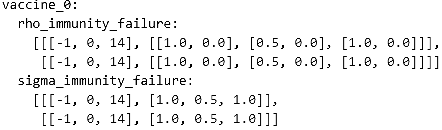
\includegraphics[width=0.5\textwidth]{codeexample2bw}
\end{center}
Here the vaccine \texttt{vaccine{\_0}} encodes updates to rho and sigma immunity for two strains of the pathogen. The updates follow the exact same multiplicative procedure as the immunity updates resulting from an infection, as described in Section \ref{sec:health}. The model also features age-dependent vaccine hesitancy, and a minimum time between doses. The input component specifies how many doses of each vaccine are available in each region each day, for each age group, with this number of doses being administered to a randomly selected subset of all eligible and willing agents.

\section{Seasonality}

The seasonal effects component of the Pandemia simulator can be used to configure monthly updates to the regional transmission multipliers. The default seasonal effects model calculates a transmission multiplier for each country each month. The default value of these multipliers is $\texttt{1.0}$, meaning no reduction in transmission. The alternative value is a float taking values in the range $\texttt{[0,1]}$. The months during which transmission is reduced to this value are configured in a data file.

\section{Travel}

The travel model implements mixing between regions. At the beginning of each day, a number of uninfected agents are randomly selected to travel from each region to each other region.

The input component associated to each region for each day a multiplier in the range $\texttt{[0,1]}.$ This multiplier represents the extent to which travel \textit{out} of the region is reduced by border restrictions that day, with the value $\texttt{0}$ representing total suppression of travel out of the country. The number of agents travelling between regions $i$ and $j$ is therefore given by the corresponding entry in the \textbf{Travel Matrix}, multiplied by the border closure multiplier of region $i$.

Travellers mix homogeneously with the entire population of the destination region. In particular, for each region $j$, an aggregated level of infectiousness is calculated, with this resulting probability, $p_j$, being calculated as:
\begin{equation*}
p_j := \left(1 - \prod_{m \in j} (1 - g_m)\right)
\end{equation*}
where $m \in j$ means all agents $m$ currently in location $j$, with
\begin{equation*}
g_m  := \omega_m\, \nu_m\, \mu(j)\, \beta(s_m)\, \tau\, /\, N_j.
\end{equation*}
where these parameters are defined as in the default health model with
\begin{itemize}
\item $N_j$ the number of agents in region $j$;
\item $\tau$ is a control parameter.
\end{itemize}
For each uninfected agent $n$ travelling to region $j$, with current face mask multiplier $\omega_n$, the probability that they are exposed at this time is then assumed to be $\omega_n p_j$. If such an agent is exposed, then to determine which strain they are exposed to, we assume the expression
\begin{equation*}
\frac{\sum_{\{m \in j: s_m = s\}} g_m}{\sum_{\{m \in l\}} g_m}
\end{equation*}
gives the probability that they are exposed to strain $s$. Given this exposure, the probability that they are actually infected with strain $s$ is then $\sigma_{ns}$, the current sigma immunity of agent $n$ against strain $s$. The outcome of this infection is then determined by the rho immunity of the agent, according the procedure outlined in the section on the default health model.

The current region of an agent $\texttt{n}$ is recorded by the variable $$\texttt{current{\_}region[n]}.$$ Agents whose current region is not their home region are considered travellers, and are ignored by other components where appropriate for the remainder of the day.

\section{Examples: World Factories and Scenarios [TO DO]}

All parameters, including the scale factor and random seed, are configured in a single file, called the \textbf{Configuration}. The choice of world factory is specified in the configuration. Several example world factories have been provided, in particular the homogeneous mixing example $\texttt{Global}$ and the heterogeneous mixing example $\texttt{Global{\_}Grid}$.

\subsection{Homogeneous World}

\begin{center}
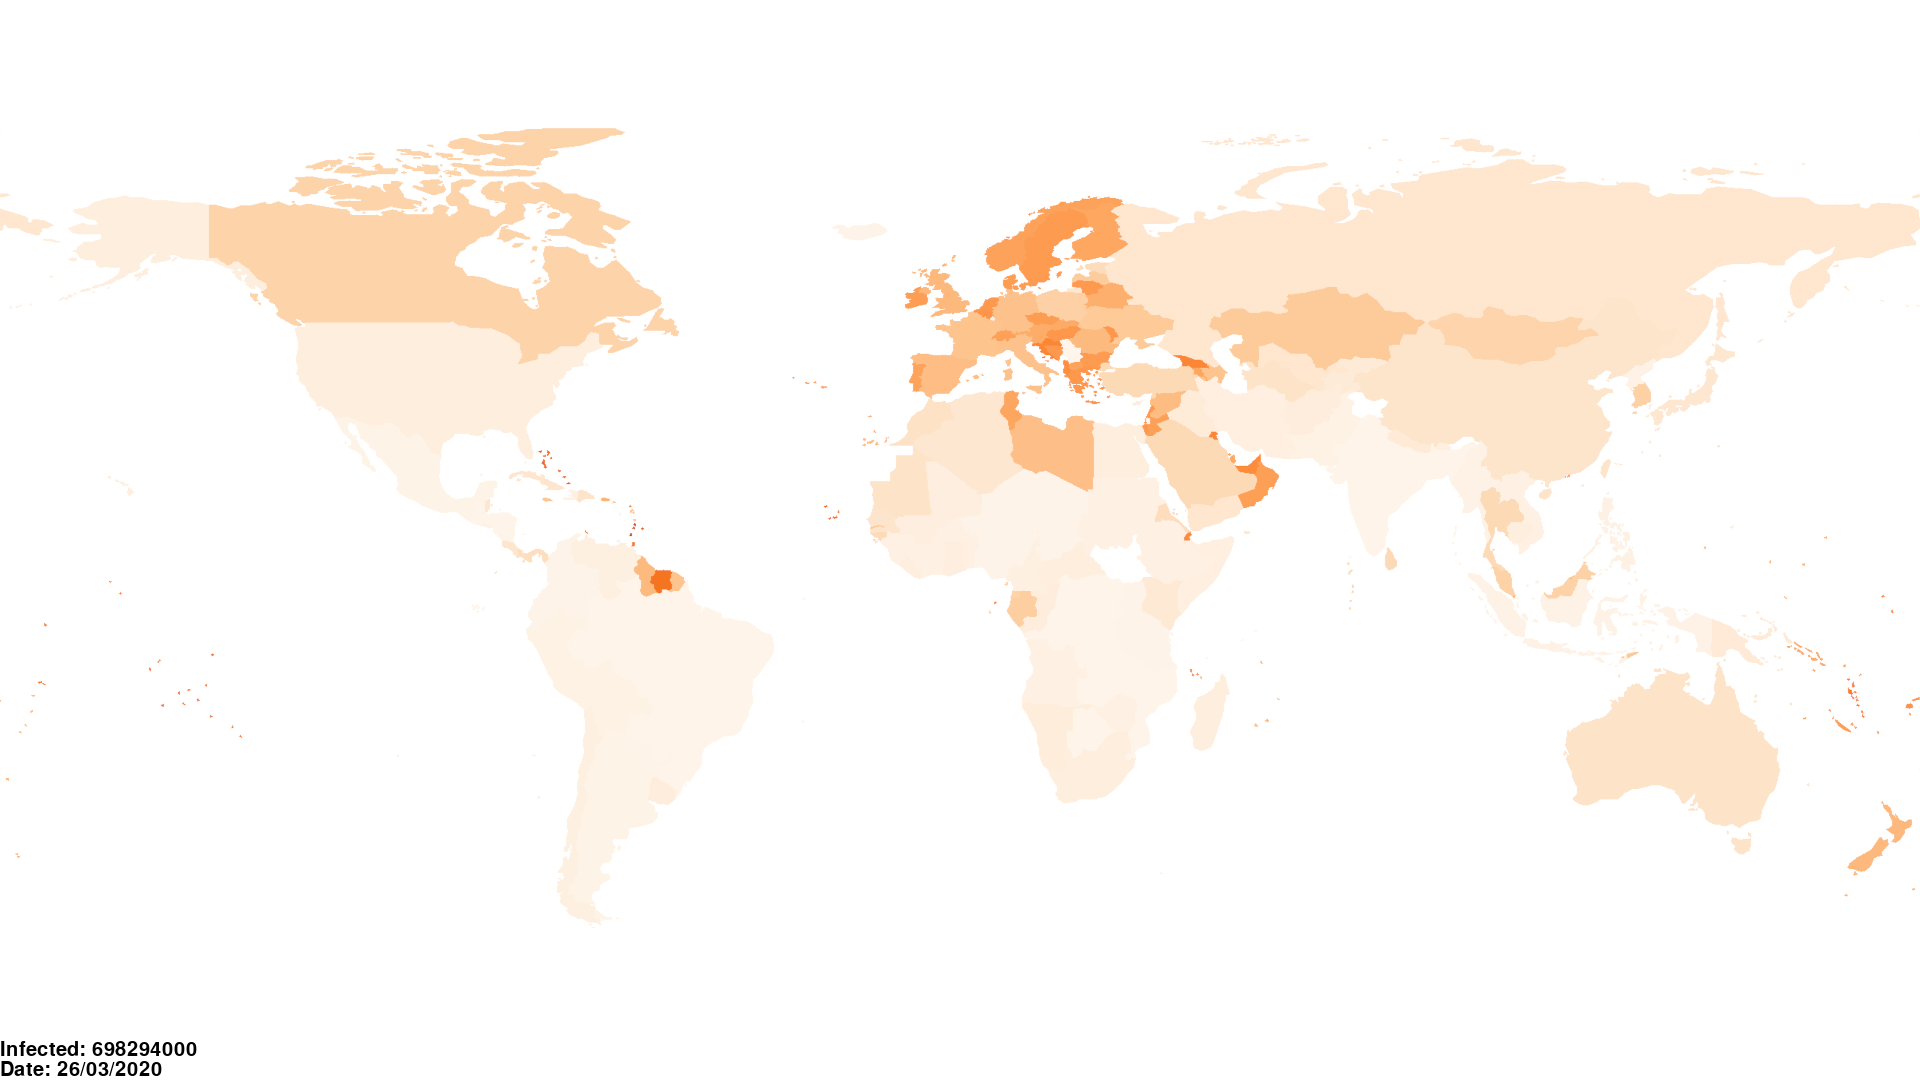
\includegraphics[width=0.9\textwidth]{homogeneous}
\end{center}

\subsection{Heterogeneous World}

\begin{center}
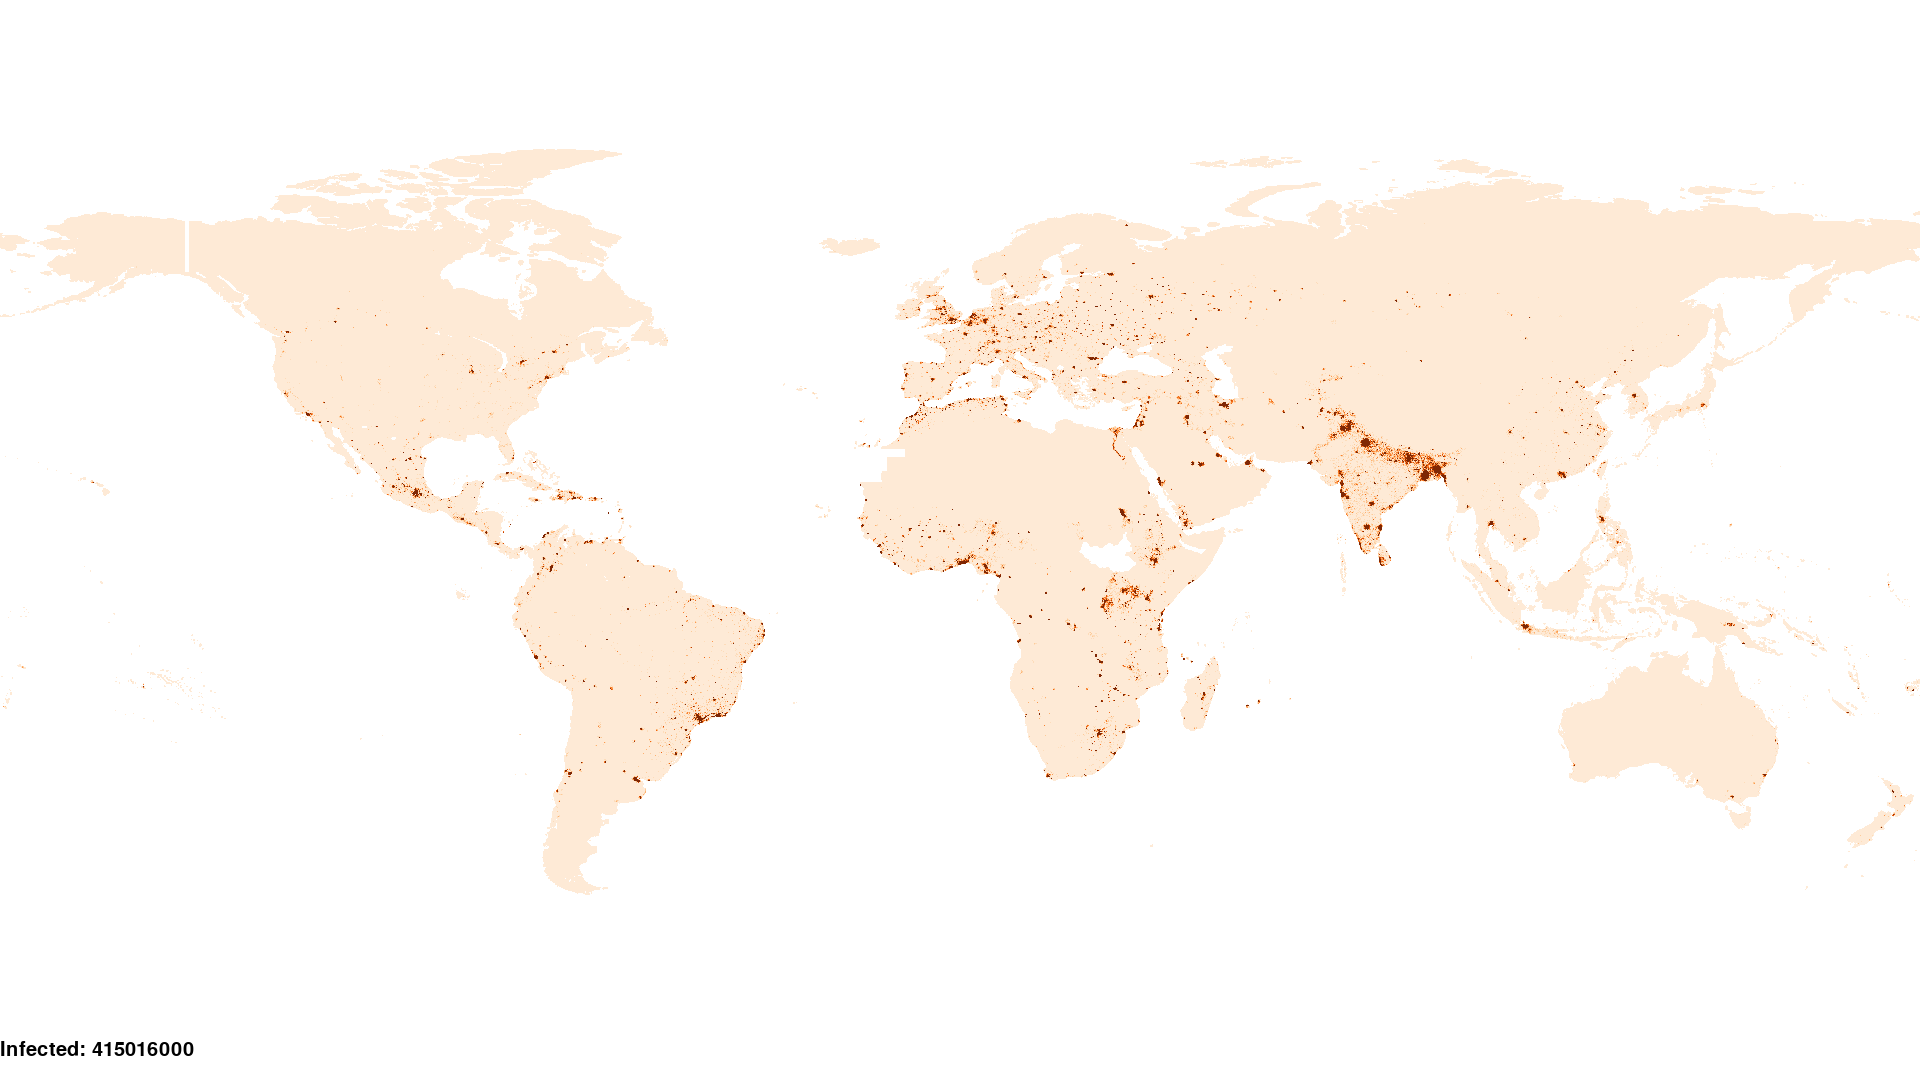
\includegraphics[width=0.9\textwidth]{heterogeneous}
\end{center}

\section{Validation}

The validation of any individual-based epidemic model can be challenging, due to the computational burden of such models. Pandemia is fast, facilitating validation methods that require rapid iteration of the model. Such validation tools can be found in the codebase, although they are currently a work in progress.

\section{Optimization}

A common approach in epidemic modelling is to propose a small number of potential control strategies, before simulating each of them to determine which is most effective. Pandemia supports a more systematic approach, based on optimization algorithms.

Recall that the world and model components are specified using a \textbf{Configuration}. Given both a \textbf{Configuration} and a \textbf{Policy}, the simulation returns a \textbf{Cost}:

$$\textbf{Cost} = \text{Sim}(\textbf{Configuration}, \textbf{Policy}).$$

For a given \textbf{Configuration}, optimization algorithms can then be used to determine the \textbf{Policy} that minimizes the \textbf{Cost}. Recall that the \textbf{Policy} is the object referred to in Section \ref{sec:input}, consisting of arrays of integers and floats, that determines which interventions are active or available in each region each day.

Such an optimization algorithm can be found in the Pandemia codebase. It uses a genetic algorithm to search for optimal policies. Much like the validation tools, this is also a work in progress.

Once these optimization algorithms are able to establish a mapping from a sample of configurations to a set of optimal policies, then methods from machine learning could be used to learn the remainder of this function.

Pandemia is able, via these optimization methods, to reveal potentially very effective control strategies that, due to the complexities of the system, may not be obvious to the modeller. Such strategies could save lives and reduce the cost of interventions. By inverting the cost function, Pandemia can also be used to determine which strategies are best avoided.

% \bibliography{bibliography}

\end{document}